\documentclass[tikz,border=4pt]{standalone}
\begin{document}
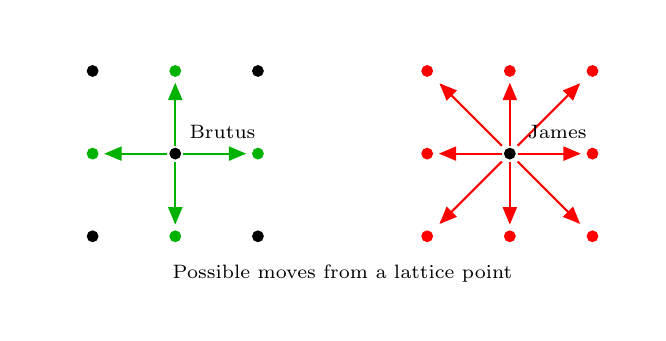
\begin{tikzpicture}[x=.025cm,y=-.025cm]
\path[use as bounding box] (0,0) rectangle (310,145);
\path[draw=black,fill=black] (33,22) circle[radius=0.0675cm];
\path[draw=green!70!black,fill=green!70!black] (33,64) circle[radius=0.0675cm];
\path[draw=green!70!black,fill=none,line width=0.77pt] (71,64) -- (40,64);
\path[draw=green!70!black,fill=green!70!black,line width=0.55pt] (40,64) -- (47.3685,60.8847) -- (47.3685,67.1153) -- cycle;
\path[draw=black,fill=black] (33,106) circle[radius=0.0675cm];
\path[draw=green!70!black,fill=green!70!black] (75,22) circle[radius=0.0675cm];
\path[draw=green!70!black,fill=none,line width=0.77pt] (75,60) -- (75,29);
\path[draw=green!70!black,fill=green!70!black,line width=0.55pt] (75,29) -- (78.1153,36.3685) -- (71.8847,36.3685) -- cycle;
\path[draw=black,fill=black] (75,64) circle[radius=0.0675cm];
\path[draw=green!70!black,fill=green!70!black] (75,106) circle[radius=0.0675cm];
\path[draw=green!70!black,fill=none,line width=0.77pt] (75,68) -- (75,99);
\path[draw=green!70!black,fill=green!70!black,line width=0.55pt] (75,99) -- (71.8847,91.6315) -- (78.1153,91.6315) -- cycle;
\path[draw=black,fill=black] (117,22) circle[radius=0.0675cm];
\path[draw=green!70!black,fill=green!70!black] (117,64) circle[radius=0.0675cm];
\path[draw=green!70!black,fill=none,line width=0.77pt] (79,64) -- (110,64);
\path[draw=green!70!black,fill=green!70!black,line width=0.55pt] (110,64) -- (102.6315,67.1153) -- (102.6315,60.8847) -- cycle;
\path[draw=black,fill=black] (117,106) circle[radius=0.0675cm];
\node[inner sep=0pt,font=\scriptsize] at (99,53) {Brutus};
\path[draw=red,fill=red] (203,22) circle[radius=0.0675cm];
\path[draw=red,fill=none,line width=0.77pt] (241,60) -- (210,29);
\path[draw=red,fill=red,line width=0.55pt] (210,29) -- (217.4132,32.0074) -- (213.0074,36.4132) -- cycle;
\path[draw=red,fill=red] (203,64) circle[radius=0.0675cm];
\path[draw=red,fill=none,line width=0.77pt] (241,64) -- (210,64);
\path[draw=red,fill=red,line width=0.55pt] (210,64) -- (217.3685,60.8847) -- (217.3685,67.1153) -- cycle;
\path[draw=red,fill=red] (203,106) circle[radius=0.0675cm];
\path[draw=red,fill=none,line width=0.77pt] (241,68) -- (210,99);
\path[draw=red,fill=red,line width=0.55pt] (210,99) -- (213.0074,91.5868) -- (217.4132,95.9926) -- cycle;
\path[draw=red,fill=red] (245,22) circle[radius=0.0675cm];
\path[draw=red,fill=none,line width=0.77pt] (245,60) -- (245,29);
\path[draw=red,fill=red,line width=0.55pt] (245,29) -- (248.1153,36.3685) -- (241.8847,36.3685) -- cycle;
\path[draw=black,fill=black] (245,64) circle[radius=0.0675cm];
\path[draw=red,fill=red] (245,106) circle[radius=0.0675cm];
\path[draw=red,fill=none,line width=0.77pt] (245,68) -- (245,99);
\path[draw=red,fill=red,line width=0.55pt] (245,99) -- (241.8847,91.6315) -- (248.1153,91.6315) -- cycle;
\path[draw=red,fill=red] (287,22) circle[radius=0.0675cm];
\path[draw=red,fill=none,line width=0.77pt] (249,60) -- (280,29);
\path[draw=red,fill=red,line width=0.55pt] (280,29) -- (276.9926,36.4132) -- (272.5868,32.0074) -- cycle;
\path[draw=red,fill=red] (287,64) circle[radius=0.0675cm];
\path[draw=red,fill=none,line width=0.77pt] (249,64) -- (280,64);
\path[draw=red,fill=red,line width=0.55pt] (280,64) -- (272.6315,67.1153) -- (272.6315,60.8847) -- cycle;
\path[draw=red,fill=red] (287,106) circle[radius=0.0675cm];
\path[draw=red,fill=none,line width=0.77pt] (249,68) -- (280,99);
\path[draw=red,fill=red,line width=0.55pt] (280,99) -- (272.5868,95.9926) -- (276.9926,91.5868) -- cycle;
\node[inner sep=0pt,font=\scriptsize] at (269,53) {James};
\node[inner sep=0pt,font=\scriptsize] at (160,125) {Possible moves from a lattice point};
\end{tikzpicture}
\end{document}
